%
% $Id: thesis_sample.tex,v 1.9 2011/12/08 02:48:59 fukuyasu Exp $
%
\documentclass[11pt]{jreport}
\usepackage{ksu_cse_thesis}
\usepackage{indentfirst}
\usepackage[dvipdfmx]{graphicx}  % ←graphicx.styを用いてEPSを取り込む場合有効にする
\usepackage{algorithm}
%\usepackage{algorithmic}
\usepackage{algorithmicx}
\usepackage{algpseudocode}
\usepackage{here}
			% 他のパッケージ・スタイルを使う場合には適宜追加
% 図とキャプションの間のスペース
\setlength\abovecaptionskip{0cm}

\newlength{\myheight}
\setlength{\myheight}{1.0cm}

\algnewcommand{\Initialize}[1]{
  \State \textbf{Initialize:}
  \State \hspace*{\algorithmicindent}\parbox[t]{0.8\linewidth}{\raggedright #1}
}

%%%%%%%%%%%%%%%%%%%%%%%%%%%%%%%%%%%%%%%%%%%%%%%%%%%%%%%%%%%%%%%%%%%%%%%%

%%
%% 主に表紙を作成するための情報
%%

%%  タイトル(修論の場合は英語表記も指定)
\title{カッコウ探索を用いた\\
アドホックネットワーク上の複製配置}
%% 英文タイトル(修論では必須)       
%\etitle{Replication Placement on Ad-hoc Network\\
	% Using Cuckoo Search}

%%  著者名(修論の場合は英語表記も指定)
\author{黒川 岳児}
%%英語著者名(修論では必須)
%\eauthor{Kentaro Hayashibara}

%%指導教員名
\supervisor{林原 尚浩}
%%英語指導教員名(修論では必須)
%\esupervisor{Naohiro Hayashibara}

%% 卒業論文・修士論文(以下のどちらかを選択)
\bachelar	% 卒業論文(4年生用)
%\master  	% 修士論文(M2用)

%%  学科・クラスタ
%\department{コンピュータサイエンス}
\department{ネットワークメディア}
%\department{インテリジェントシステム}

%%  学籍番号
\studentid{544520}

%%  卒業年度
\gyear{2018}		% 提出年が2011年なら,2010年度

%%  論文提出日
\date{2019年1月23日}	% 修士の場合は月(2011年2月等)までとし,英語表記も指定
%\edate{February 2011}


%%%%%%%%%%%%%%%%%%%%%%%%%%%%%%%%%%%%%%%%%%%%%%%%%%%%%%%%%%%%%%%%%%%%%%%%

\begin{document}

\maketitle

%%
%%  概要
%%
\begin{abstract}
参加ユーザ間での通信・やり取りが行われる,Peer to Peer(P2P)ネットワークは,データ共有や分散ストレージ等,幅広い用途で使用される.今回,P2Pネットワークと性質が似ている,アドホックネットワークを,災害時に携帯端末で構成し,物資補給情報や復旧情報,個人の避難情報等のデータがやり取りされる状況を想定した.個人の避難情報は必要とする人が比較的少なくデータ要求数が少ないが,必要とする人が必ずいるため,必要性が高い.しかし,既存の主な複製配置手法では,データ要求数の少ないデータはネットワークから消失しやすいため,必要性の高いデータであっても,ネットワークに生存し続けることは出来ない.そこで,本研究では,データ要求数の少ないデータのネットワークでの生存を考慮した複製配置を提案する.複製配置先の選出には,メタヒューリスティックアルゴリズムである,カッコウ探索を用いる.そして,本提案手法と,関連研究の提案手法,既存複製配置手法の,データの生存数の推移と,全ノードのストレージ占有率の平均の推移の比較を行った.また,本提案手法と,関連研究の提案手法で行こなわれる,データ要求数の少ないデータの複製配置で,実際に配置したノードのパラメータの統計の平均値の比較を行った.
\end{abstract}

%%  目次
\tableofcontents

%%  図目次 (図目次をいれたければ以下のコメントをはずす)
\listoffigures

%%  表目次 (表目次をいれたければ以下のコメントをはずす)
\listoftables

\newpage
\pagenumbering{arabic}	% 以降のページ番号を算用数字に

%%%%%%%%%%%%%%%%%%%%%%%%%%%%%%%%%%%%%%%%%%%%%%%%%%%%%%%%%%%%%%%%%%%%%%%%

%%
%%  本文はここから
%%

\chapter{はじめに}
\section{背景}
近年,ネットワークインフラの普及により,多くの端末がインターネットに接続するようになった.そのため,従来の,ユーザとサーバが通信してやり取りを行う,クライアントサーバ方式では,サーバ側の負担が大きくなる.そこで,ユーザ同士で通信しやり取りを行う,Peer to Peer(P2P)ネットワークが注目されている.
\par P2Pネットワークは,参加ピア間でのデータ共有,耐故障性の向上のため,複数のピアにデータを配置する等,幅広い用途で使用されている.これらのP2Pネットワークで扱われるデータのデータ要求数は一様ではなく,データごとに大きく異なる可能性がある.
\par P2Pネットワークでは,データ要求が発生すると,データの検索が行われ,検索が成功すると,データの複製が作成され,データ要求者に複製が配置される.現在,主な複製配置手法では,データ要求数の多いデータの複製は多く作成されるが,データ要求数の少ないデータは作成される複製が少ない.複製が少なければ,ユーザによる削除や,ユーザのP2Pネットワークからの離脱により,データがP2Pネットワークから消滅してしまう可能性が高くなる.
\par ここで,データ要求数の少ないデータの必要性や重要性が高い場合を想定する.この場合,データ要求数が少ないデータであっても,P2Pネットワークに長期間データを生存させ続ける必要がある.しかし,前述の通り,現在の主な複製配置手法では,データ要求数の少ないデータはP2Pネットワークから消滅しやすい.その為,データ要求数の少ないデータの生存を考慮した複製配置手法が必要である.
\par そこで,今回,災害時に携帯端末で構成されるアドホックネットワークで,物資補給情報や復旧情報,個人の避難情報等のデータがアップロードされる状況を想定する.アドホックネットワークはP2Pネットワークと特徴,ネットワークトポロジが似ており,参加ユーザ間での通信,やり取りが行われる.ネットワークにアップロードされるデータの中で,個人の避難情報は,家族や親戚,友人等,数人〜数十人程度の,比較的少数の人から必要とされると考えられ,物資補給情報や復旧情報等に比べ,データ要求数が少ないと考えられる.しかし,避難情報は,家族や親戚,友人等,必ず必要とする人がいると考えられ,必要性が高いと考えられる.このケースを考慮し,データ要求数の少ないデータを長期間,アドホックネットワークに生存させる手法を提案する.

\section{問題点}
前述したよう,現在の主な複製配置手法は,必要性や重要度の高いデータであっても,データ要求数が少なければ,作成される複製数は少なく,P2Pネットワークから消滅しやすい.

\section{目的}
データ要求数の少ないデータが,P2Pネットワーク上で一定期間生存することができるよう,データ要求数の少ないデータを考慮した複製配置手法を提案し,既存の主な複製配置手法と,関連研究との比較を行う.比較内容は,データの生存数(複製数)の推移と,全ノードのストレージ占有率の平均の推移である.

\section{論文構成}
本論文は次のように構成する.第2章では,既存のP2Pネットワークの検索・複製配置手法の説明と,問題点の提示を行う.第3章では,関連研究の説明と,問題点の提示を行う.第4章では,本研究で用いたアドホックネットワークの説明と,アドホックネットワークのモデルとして用いたRandom Geometric Graphの説明を行う.第5章では,本研究で提案する,カッコウ探索を用いた複製配置手法の説明と,カッコウ探索のアルゴリズムの改変について説明する.第6章では,シミュレーションに用いた「PeerSim」の説明と,シミュレーションシナリオの説明,シミュレーション結果・考察を行う.第7章では,本研究のまとめと,今後の課題について説明する.



\chapter{既存の検索・複製配置手法}
本章では,非構造P2Pネットワークの既存のデータ検索手法と,複製手法の説明を行い,問題点を提示する.

\section{検索手法}
検索手法は,目的のデータを持つピアを発見するため,データを要求するピアが送信する検索要求メッセージの転送手法を指す.以下の検索手法が提案されている\cite{maruta}.

\begin{itemize}
	\item {\tt Flooding}
	\par データ要求するピアは,自身の全ての隣接ピアに検索要求メッセージを転送する.検索要求メッセージを受け取ったピアは,該当データを持っていない場合,同様に検索要求メッセージを自身の全ての隣接ピアに検索要求メッセージを転送する.
	\par 検索要求メッセージにはTTL(Time To Live)が設けられており,検索要求メッセージが隣接ピアに転送されるごとに値が1つ減る.値が0になった場合は,データを発見することができなかったと判断され,検索失敗となる.
	
	\item {\tt Expanding Ring}
	\par TTLの値を小さく設定し,Floodingによる検索を開始する.検索に失敗した場合,TTLの値を増加させ,再びFlooadingによる検索を行う.TTLがあらかじめ設定した上限値に達した場合は検索失敗となる.
	
	\item {\tt k-walker random walk}
	\par データを要求するピアは,k個の検索要求メッセージを自身の隣接ピアにランダムに転送する.検索要求メッセージを受け取ったピアは検索要求メッセージごとに隣接ピアの内からランダムに一台選択し,検索要求メッセージを転送する.TTLが設けられており,TTLが0になった場合は検索失敗となる.
\end{itemize}

\section{複製配置手法}
複製配置手法は,データを要求するピアが送信する検索要求メッセージが,目的のデータを持つピアに届き,検索が成功した場合に,検索の過程で得られた情報を基に複製を配置する際に用いられる手法を指す.以下の複製配置手法が提案されている\cite{maruta}.

\begin{itemize}
  \item {\tt Owner Replication}
  \par データ要求したピアにのみ複製を配置する。

  \item {\tt Path Replication}
  \par 検索対象のデータを持つピアから,データ要求したピアに至るまでの経路上にあるすべてのピアに複製を配置する.

  \item {\tt Random Replication}
  \par 検索対象のデータを持つピアから,データ要求したピアに至るまでの経路上にあるピアと同数のピアをネットワーク上からランダムに選び,複製を配置する.
\end{itemize}

\section{問題点}
既存複製配置手法は,データ要求があったデータの複製を配置する手法であるため,需要の高いデータは多くの複製が作成される.複製が多いと,そのデータへのデータ要求が成功しやすくなり,ネットワークの多くのピアでやり取りされる。
\par 一方,需要の低いデータは,データ要求が少なく,複製が作成されにくい.複製が少ないと,ユーザによる複製の削除や,複製を持っているピアの離脱により,ネットワークからデータが消滅しやすくなる.
\par このように,既存複製配置手法は,需要の高いデータを効率よくネットワークに広めることを目的としており,需要の低いデータの生存を考慮していない.



\chapter{関連研究}
本章では,影山ら\cite{kageyama}によって提案された手法の説明と,問題点の提示を行う.

\section{提案手法}

\subsection{概要}
影山らは,スーパーノード型P2Pネットワークにおける低需要データの消失を防ぐ複製配置手法を提案した.データ要求数を需要とし,各データの需要予測を行い,データが低需要データか判定する.低需要データではないデータのデータ要求があり,検索が成功した場合,Owner Replicationにより複製配置する.低需要データであり,データ要求がない場合,提案手法による複製配置数を行う.複製配置個数は需要予測により決定され,複製配置先ノードはノードの信頼度を元に配置する.

\subsection{スーパーノード型P2Pネットワーク}
スーパーノード型P2Pネットワークは,ネットワークにサーバを含まないネットワークであり,スーパーノードと一般ノードから構成される.スーパーノードは自身と,その配下の一般ノードを1グループとし,スーパーノード同士でネットワークを形成する.
\par スーパーノードは,ネットワーク上の高性能なノード群が担い,スーパーノード配下の一般ノードに関するデータを持つ.データの探索はスーパーノードが行い,データの取得は一般ノード同士で直接行う.スーパーノード配下の一般ノードに関するデータをスーパーノードで集中管理するため,探索速度が速い,システムの管理・制御が可能といった特徴を持つ.

\subsection{需要予測}
$データ要求数を需要とし、需要の変動はポアソン過程に従うと仮定する.ある時刻tにおける需要d(t)は次のように表される.\lambda は単位時間中の平均のデータ要求数を示す.$

\[
d(t)=\frac{e^{-\lambda}\lambda^t}{t!}
\]

\par $単位時間毎にデータへの需要を計測し,指数平滑法に基づく需要予測を行う.時刻tにおける需要の実測値をMd_t,Fd_tと表す.この時,需要予測値Fd_{t+1}は次のように表される.$

\[
Fd_{t+1}=\alpha \times Md_t+(1-\alpha) \times Fd_t
\]

\par $\alpha は平滑係数を示す.提案手法では,Fd_{t+1}<0.05となるデータは低需要データと判断され,複製配置処理が行われる.$

\subsection{複製配置}
複製配置個数は現在のデータ数,需要予測値,実測値の比から求める.$時刻tでのファイル数をN_t,安全数をS_tとすると,複製配置個数は次のように表される.$

\[
S_t=\beta \times N_t \times \frac{Fd_{t+1}}{Md_t}
\]

\par $\beta$ は安全係数を示す.複製配置先ノードは,貢献度と生存率という2つの基準を用いて選出する.
\par 貢献度は,データのやり取りにどれだけ貢献してきたかを示す度合いである.貢献度はデータのアップロード(UL)回数,ダウンロード(DL)回数,平均稼働時間から決定すし,次のように表される.

\[
貢献度=\frac{UL回数}{UL回数+DL回数} \times 平均稼働時間
\]

\par 生存率はユーザがサービスを利用する頻度を推定する.次の3つの仮定を利用し,生存率を決定する.

\begin{itemize}
	\item {\tt 仮定1:ユーザの生存期間は指数分布に従う}
	\par 生存期間はユーザがサービスを利用する意思のある期間を示す.ユーザのサービスからの離脱は,過去の生存期間に関わらずランダムに発生するとする.生存期間を$\tau$とすると,ユーザの生存期間$f(\tau)$の確率分布は次のように表される.
	
	\[
	f( \tau )= \mu e^ {-\mu \tau}
	\]
	
	\item {\tt 仮定2:DL,ULはポアソン過程に従う}
	\par DLとULは,過去にいつ起きたかに関わらずランダムに発生すると仮定する.$\tau$期間以上生存したユーザの$T$期間のDLとULの回数$x$の確率は次のように表される.
	
	\[
	P(x| \nu,\tau>T)=\frac{(\nu T)^x}{x!} \times e^{- \nu T}
	\]
	
	$\nu$はポアソン過程のパラメータであり,単位時間あたりのDLとULの頻度を示す.
	
	\item {\tt 仮定3:生存期間の分布$\mu$とDL,ULの頻度の分布$\nu$はユーザごとに異なる}
\end{itemize}

\par 以上の3つの仮定より,生存期間$\tau$がTより大きくなる確率,すなはち,計測終了時点でユーザが生存していることを表す生存率は次のように表される.

\[
p(\nu, \mu, \tau, T, t)=\frac{1}{1+ \frac{\mu}{\nu + \mu} [e^{(\nu + \mu)(T-t)} -1] }
\]

\par $t$は初回から最後のDLまたはULまでの期間を示す.$T$は初回のDLまたはULから計測終了までの期間を示す.

\section{問題点}
影山ら\cite{kageyama}の研究では,スーパーノード型P2Pネットワーク上での複製配置を提案している.しかし,今回提案する手法で用いるコンピュータは携帯端末であり,端末ごとの性能に大きな差は生じにくい.そのため,今回の提案手法では,スーパーノード型P2Pネットワークではなく,アドホックネットワークを用いた複製配置を行う.
\par また,影山ら\cite{kageyama}の研究では,低需要と判定されたデータの複製をネットワークに生存させ続けるという手法であるため,ネットワークにアップロードされるデータの種類が増えていくと,ストレージの使用量も線型的に増加し続ける.そのため,今回の提案手法では,低需要データと判定され,複製配置を開始後,一定期間経過するまでに,一度もデータ要求がない場合,複製配置を取りやめるという方法を取る.



\chapter{ネットワークモデル}
本章では,本研究で用いるアドホックネットワークと,アドホックネットワークのモデルとして用いた,Random Geometric Graphの説明を行う.

\section{アドホックネットワーク}
アドホックネットワークは,PC,PDA,携帯電話といった無線で接続できる端末のみで構成されたネットワーク形態のことで,必要に応じてダイナミックなネットワークシステムの構成が可能である.各端末がデータを中堅することが可能であり,端末間をリレー方式で接続することにより,これまで線の繋がりであったネットワークを,面でつなぐことが可能となった.そのため,災害時に,不通となってしまった地域で,アドホックネットワークを構築することにより,柔軟かつ迅速に通信インフラを確保するといったことが可能となる\cite{nomura}.

\section{Random Geometric Graph}
Random Geometric Graphは$G(n, r)$に従う.$n$個の頂点を2次元平面上に一様ランダムに配置する.頂点は通信半径$r$持っており,2つの頂点間の距離が$r$以下であれば,相互に辺を貼る\cite{jesper}.図\ref{fig:rgg}にRandom Geometric Graphの例を示す.

\begin{figure}[htbp]
	\begin{center}
		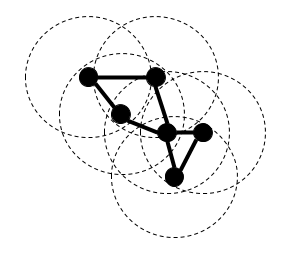
\includegraphics[width=5.0cm]{./figure/rgg.png}
	\end{center}
	\caption{Random Geometric Graphの例}
	\label{fig:rgg}
\end{figure}

\par Random Geometric Graphの通信半径$r$の値を定めるために,Philipsら\cite{thomas}の研究で定められた,連結性を保つためのノードの通信半径$r$を求める式\ref{exp:r}を用いる.

\begin{equation}
r=\sqrt{ \frac{(1+\epsilon)\ln{A}}{D\pi}}, \epsilon>0 \label{exp:r}
\end{equation}

$D$は単位領域におけるノード数を示しており,$D=\frac{N}{A}$.$N$はノードの数,$A$は2次元領域の大きさを示している.



\chapter{提案手法}
本章では,低需要データを一定期間,アドホックネットワーク上に生存させ続けるための複製配置手法を提案する.提案手法の概要,データの需要について,低需要データの複製配置先・複製個数について,低需要データを複製配置するために用いるカッコウ探索の説明を行う.

\section{概要}
本提案手法では,先ず,各ノードがデータ要求確率に基づきデータ要求を行う.データ要求を行うノードは,目的のデータを検索し,検索が成功すれば,自身に複製を配置する.全てのノードのデータ要求が完了後,アドホックネットワーク上の,各データごとの複製数を計測する.ここで,低需要データの判定を行い,低需要データと判定されれば,カッコウ探索を用いた複製配置が行われる.

\section{データの需要}
\subsection{データ要求}
各ノードは,各データごとに,データ要求をする確率(データ要求確率)を持っている.データ要求確率はポアソン分布に従い変動すると仮定する.データ要求確率は次のように表される.

\begin{equation}
P(X=k)=\frac{\lambda^{k}e^{-\lambda}}{k!} \label{exp:data}
\end{equation}

この式\ref{exp:data}は,単位時間に$\lambda$回発生するデータ要求が,$k$回発生する確率を表す.
\par データ要求確率に従い,データ要求が発生すると,Floodingによる検索要求メッセージの転送が行われる.検索要求メッセージが$TTL>0$の間に,該当データを所持するノードに到達すると,検索が成功する.その後,Owner Replicationにより,データ要求したノードに複製が配置される.複製にはTTLが設定されており,時間経過で1づつ減っていく.この値が0になると,ユーザによる複製の削除が発生すると仮定する.本稿では,複製数を需要とする.

\subsection{低需要データ}
低需要データの複製配置を行うためには,各データごとに,データが低需要データであるのか判定する必要がある.その為,全てのノードのデータ要求が完了した後,アドホックネットワーク上の,各データごとの需要を計測する.ここで,以下の2つの条件を満たすデータは,低需要データとして扱うこととする.

\begin{itemize}
	\item {\tt 条件1:あるデータの需要が,全種類のデータの全需要の5%以下である}
	
	\begin{equation}
	R_i \le 0.05 \times \sum_{i=0}^{n-1} R_i
	\end{equation}
	
	$R_i$はデータ$i$の複製数,$n$はデータの種類の数を示している.
	\item {\tt 条件2:あるデータの現在の需要が,そのデータの最大需要と比較し,減少している}
	
	\begin{equation}
	R_i < \max{(R_i)}
	\end{equation}	
	
	$max(R_i)$はデータ$i$の最大複製数を示している.この条件は,需要が減少していることを示している.
\end{itemize}

\par 低需要データを複製配置するにあたり,複製配置先の決定と,複製配置個数の決定を行う,

\section{複製配置先,複製個数の決定}
各ノードは,バッテリー残量とストレージ残量を持っていると仮定する.そこで,本提案手法の複製配置先の決定には,バッテリー残量とストレージ残量の2つの評価を用いる.評価式は次式を用いる.

\begin{equation}
評価値 = \alpha \times \frac{現在のバッテリー残量}{最大バッテリー容量} + \beta \times \frac{現在のストレージ残量}{最大ストレージ容量} 
\end{equation}

$\alpha$,$\beta$は重みを表す.今回は,最大バッテリー容量は100.0,最大ストレージ容量は10.0とする.
\par バッテリー残量の高いノードは,バッテリー切れでアドホックネットワークから離脱する可能性が低く,ノードの離脱による複製の削除が発生しづらくなる.また,ストレージ残量の高いノードに割り当てることにより,特定のノードのストレージへ複製が集中する状況を避けられ,1つのノード離脱による,多数の複製の削除が発生しづらくなる.
\par 低需要となったデータの複製は,データがアドホックネットワークに生存し続けられる程度で良い.そこで,本提案手法では,低需要データの複製を少なくとも5個,アドホックネットワークに生存させ続ける.また,ストレージ節約のため,複製配置を開始後,一定期間経過する間に,一度もデータ要求ない場合,複製配置を取りやめる,という手法を取る.
\par 低需要データと判定されたデータは,データ要求による複製配置とは別に,カッコウ探索を用いて,上記の評価指標が優れているノードを選び,複製配置を行う.

\section{カッコウ探索による複製配置}
本提案手法では,低需要と判定されたデータを,カッコウ探索を用いて複製配置する.

\subsection{カッコウ探索}
カッコウ探索(Cuckoo Search)は,YangとDebによって2009年に提案された,連続値最適化問題を対象とした,メタヒューリスティックアルゴリズムである\cite{yang1}\cite{yang2}.
\par カッコウは,他種の鳥の巣に卵を産み付け,育てさせる托卵という生体行動を行う.その際,産み付ける卵を,巣の主が生む卵と似せ,巣の主に気づかれにくくすることができる.しかし,巣の主に見つかってしまうこともあり,その場合,巣の主は巣を放棄し,新たな場所に巣を作るか,カッコウの卵を巣から捨てるという行動をとる.
\par カッコウ探索のアルゴリズムは,このカッコウの習性から着想を得ており,以下の3つに着目している.

\begin{itemize}
  \item {\tt カッコウは他の鳥の巣に卵を産む}
  \item {\tt カッコウが生む卵は,巣の主の卵に似ている}
  \item {\tt 時には巣の主が托卵に気づき,巣の放棄をする}
\end{itemize}

\par カッコウの目標は,托卵を巣の主に気づかれることなく,自分の卵が孵り,巣立つまで,巣の主に育ててもらうことである.そこで,カッコウ探索では,巣の主に気づかれない卵を「良い卵」,良い卵のある巣が「良い巣」であると考える.問題に対する「解」を,巣に置かれた「卵」として表現し,巣の卵の更新と,悪い巣の放棄を繰り返し,良い卵を作り出す,世代交代をすることにより,最適解を導き出す\cite{ohtani}.
\par 巣の卵の更新と,巣の卵の廃棄は,以下の仮定に基づきモデル化する.

\begin{itemize}
	\item {\tt カッコウはLevy walkを用いて,他の巣の卵に,似た卵を産む}
    \item {\tt 托卵先の卵よりも良い卵を産んだ場合,巣の主に気づかれない}
    \item {\tt 悪い卵を持つ巣は放棄される}
    \item {\tt 托卵先の数は変化しない}
\end{itemize}

\subsection{Levy walk}
カッコウ探索では,新しい卵の生成にLevy walkを用いる.
\par Levy walkは,Paul Levyによって提案された連続空間上のランダムウォークである\cite{paul}.このランダムウォークは,向き$o$を一様ランダムに$[0, 2\pi)$から決定し,step length $d$を次式のべき分布に従って決定する.

\begin{equation}
p(d) \propto d^{ -\lambda} \label{exp:levy}
\end{equation}

ここで,$p(d)$は確率密度で,$\lambda$は,$1.0<\lambda<3.0$を領域とするパラメータである.べき分布に従うため,Levy walkは短距離の移動を続ける中,稀に長距離移動を行う.パラメータ$\lambda$が大きくなるにつれ,局所的な探索になり,$\lambda>3.0$の時,Levy walkは,ランダムウォークになると報告されている\cite{sergey}.
\par Levy walkは,アホウドリや蟻などの,動物の採餌行動であると報告されており\cite{andrew}\cite{viswanathan},広大な空間に対し,希少な資源を探すのに有効であると報告されている\cite{koyama}.
\par カッコウ探索は,連続値最適化問題を対象としているため,カッコウ探索で扱われるLevy walkもまた,連続空間上での探索を想定されている.しかし,今回の提案手法では,離散空間のRandom Geometric Graph上でLevy walkを用いる.その為,離散空間での探索を想定したLevy walkに改変する必要がある.

\subsection{Random Geometric Graph上のLevy walk}
前述の通り,Levy walkは連続空間上のランダムウォークであるため,離散空間上での探索は想定されておらず,探索手法を改変する必要がある.そこで,ここでは,Random Geometric Graph上で探索するため,Levy walkの探索方法を改変する.
\par ここで,西田\cite{nishida}によって定義された,グラフ上のLevy walkについて記す.
\par ランダムウォークによって移動する物体をエージェントと呼ぶこととする.
\par 西田\cite{nishida}によって定義された,グラフ上のLevy walkでは,初めに,向き$o$を$[0, 2\pi)$から一様ランダムに決定し,次に,step length$d$をべき分布に従って決定する.つまり,方向$o$へ$d$回,隣接頂点に遷移を行う.
\par 続いて,これをRandom Geometric Graphに適応する.Random Geometric Graphでは,頂点は2次元平面上に配置され,各頂点は2次元平面上の座標を保持しており,エージェントはそれを知ることが可能であると仮定する.これにより,頂点の接続辺に対し,向きを定義することが可能である.しかし,接続辺の繋がっている方向が各頂点ごとに同じではなく,同じ方向に進み続けることができるとは限らない.この特徴を考慮し,Random Geometric Graph用にLevy walkを定義する.
\par エージェントの状態を$(v, o ,d)$の組で表す.$v$はエージェントが現在いる頂点を表す.$o$は進む方向を表し,$[0, 2\pi)$の実数.$d$は今の方向に対し,進む距離を表し,$d>0$.エージェントは以下の手順でRandom Geometric Graph上を移動する.

\begin{enumerate}
	\item $v=$ Levy walkの出発点とする.
    \item $o$を$[0, 2\pi)$から一様ランダムに決定する.
    \item $d$をべき分布に従い決定する.$d$は式\ref{exp:levy}の確率分布に従う.
    \item $v$の接続辺の中に,その方向と$o$の成す角が閾値未満である辺が存在しなければ,$o$の方向にこれ以上進めないと判断し,2に戻る.
    \item $d=0$であれば2に戻る.そうでなければ,$d=d-1$とし,$o$に最も近い方向にある$v$の接続点を通り,移動した先の頂点を$v$とし,4に戻る
\end{enumerate}

\subsection{カッコウ探索のアルゴリズム}
カッコウ探索の基本的なアルゴリズムは,最初に初期の巣をランダムに生成する.次にランダムに選んだ巣を元に,Levy walkを用いて新しい卵を生成する.ランダムに選んだ巣の卵より,新しい卵の方が評価値が高ければ,卵を置き換える.これが托卵に相当する処理である.その後,ある一定の割合の悪い卵を持つ巣を,新しい巣で置き換える.これが,巣の主が托卵に気づき,巣を放棄することに相当する処理である.それまでに得られた最良卵を記録しつつ,上記の処理を,終了条件が満たされるまで繰り返す.終了条件には,最大世代交代数を超える,目標とする評価値以上の解を得る,最良卵が一定期間変化しない等が用いられる.以下のアルゴリズム\ref{alg:cuckoo}に,カッコウ探索のアルゴリズムを記す.

\begin{algorithm}                 
\caption{カッコウ探索のアルゴリズム}
\label{alg:cuckoo}
\begin{algorithmic}[1]

\Initialize{
   目的関数:$f(x), x=(x_1, ..., x_d)^{T};$
   \\ n個の巣を生成:$x_i (i=1, 2, ..., n);$
  }
  
\While{$(終了条件);$}
	\State 巣をランダムに選択,その巣の卵を$j$とする:
      \State 卵$j$を持つ巣を元に,Levy walkを用いて新しい卵$i$を生成;
	\State 新しい卵$i$を評価:$F_i$;
	\State ランダムに選んだ巣の卵$j$を評価:$F_j$;
    
	\If{$(F_i > F_j),$}
		\State ランダムに選んだ巣の卵$j$を,新しい卵$i$で置き換え;
      	         \State 巣の並び替え;
    \EndIf
    
    \State 一定数の割合の悪い巣を放棄し,新しい巣を生成;
    \State 巣の並び替え
\EndWhile
\State 最適解が決定

\end{algorithmic}
\end{algorithm}

\par カッコウ探索で,巣$N_r$をもとにして,Levy walkにより巣$N_i$を生成する際,$j$番目の卵の要素$x_{j}^{i}$は次式で求めることができる.

\begin{equation}
x_{j}^{i}=x_{j}^{r}+\alpha \times s \label{exp:cuckoo}
\end{equation}

ここで,$\alpha$はLevy walkの1ステップ長を調整するためのパラメータで,$\alpha>0$.$s$はLevy walkで求めるステップ長を示している.
\par カッコウ探索は連続値最適化問題を対象としている為,離散値を扱う本提案手法では,アルゴリズムの改変が必要になる.

\subsection{提案手法でのカッコウ探索のアルゴリズム}
本提案手法では,Random Geometric Graph上に配置されたノードを探索し,評価指標の優れたノードに複製を配置する.その為,Levy walkを用いて新しい巣を生成する式\ref{exp:cuckoo}を変更する.
\par 本提案手法では,卵は,ノードが保持している「バッテリー残量」と「ストレージ残量」に該当するため,新しい卵を生成することはできない.その為,本提案手法では以下の手順に従い,値の更新(托卵)を行う.

\begin{enumerate}
	\item 巣$N_i$をもとにして,Levy walkにより巣$N_j$を発見.
	\item 巣$N_i$の卵$x_i$と,巣$N_j$の卵$x_j$の評価を比較.
	\item Levy walkにより発見した巣$N_j$の方が良い巣であれば,巣$N_i$を巣$N_j$で置き換える.
\end{enumerate}



\chapter{シミュレーション}
本章では,アドホックネットワークのモデルとしてRandom Geometric Graphを実装し,低需要データを一定期間生存させるシミュレーションの説明を行う.

\section{概要}
提案手法を評価するために,P2Pネットワークシミュレータ「PeerSim\cite{peersim}」を用いた.PeerSimは,高スケーラビリティ,動的システムをサポートしている,オーバーレイネットワークシミュレータである.PeerSimは離散イベントシミュレータであり,サイクルに基づいて実行される.
\par 本提案手法とOwner Replication,Path Replication,関連研究の提案手法をPeerSimでシミュレートし,比較を行った.比較内容は以下の通りである.

\begin{itemize}
	\item {\tt サイクル毎のデータの生存数}
	\item {\tt サイクル毎の全ノードのストレージ占有率の平均}
\end{itemize}

\par 関連研究は,スーパーノード型P2Pネットワークでの提案であった.しかし,今回の比較では,アドホックネットワークを用いる.その為,関連研究では,スーパーノードを通じて評価値の高いノードを探索していたが,今回は,ランダムにノードを選び,そのノードを元にFloodingを用いて探索する手法に変更した.
\par また,カッコウ探索を用いた本提案手法と,複製配置先の探索をFloodingを用いるよう設定した関連研究の提案手法が,複製配置先として選出したノードの,バッテリー残量,ストレージ残量の比較を行う.

\section{シナリオ}
提案手法では,以下の手順で1サイクルとする.

\begin{enumerate}
	\item ノードの参加・離脱確率に従い,ノードの参加・離脱の発生.
	\item データ要求確率に従い,データ要求の発生.
	\item 需要の計測.
	\item 関連研究の提案手法と,本提案手法のみ,低需要データがあれば複製配置.
	\item 各データのTTLの減少.
	\item 各ノードが保持するバッテリー残量の減少.
\end{enumerate}

サイクルの初めに行われる,ノードの参加・離脱について説明する.
\par ノードの参加・離脱は,参加・離脱候補ノードが10個あるとし,共にポアソン分布に従い,参加・離脱確率が変動すると仮定する.ノードの参加・離脱確率は次のように表される.

\begin{equation}
P(X=k)=\frac{\lambda^{k}e^{-\lambda}}{k!} \label{exp:node}
\end{equation}

この式\ref{exp:node}は,単位時間に$\lambda$回発生するノードの参加・離脱が,$k$回発生する確率を表す.
\par ノードの参加・離脱確率に従い,ノードの参加が発生すると,新たにノードが作成され,ネットワークに追加される.参加候補ノード数は10個から変動させないため,参加したノード数分,候補ノードを追加する.
\par ノードの参加・離脱確率に従い,ノードが離脱すると,ランダムに選ばれたノードが,ネットワークから削除される.その際,保持しているデータと複製は全て削除される.離脱候補ノード数も10個から変動させないため,ノード離脱確率に従い離脱したノード数分,候補ノードを追加する.
\par ノードの離脱は,ノードの保持しているバッテリーが0以下になった場合にも発生し,バッテリーは毎サイクルごとにランダムに減っていく.

\section{環境}
PeerSimを用いて,$200 \times 200$の2次元平面に,2000個のノードを一様ランダムに配置し,Random Geometric Graph上にてシミュレーションを行う.ネットワークにアップロードされるデータの種類は全部で50種類で,5サイクルごとに,1種類のデータがアップロードされる.シミュレーションシナリオは,500サイクル分実行される.

\section{結果と考察}
はじめに,サイクル毎のデータ生存数の結果を記す.続いて,サイクル毎の全ノードのストレージ占有率の平均の結果を記す.最後に,カッコウ探索とFloodingで複製配置先に選んだノードのパラメータの平均の結果を記す.

\subsection{サイクル毎のデータ生存数}
データは全50種類であるが,結果をわかりやすくするため,図に記すのは,データ5,データ15,データ25,データ35,データ45の5個とする.
\par 図\ref{fig:owner_c}にOwner Replication,図\ref{fig:path_c}にPath Replication,図\ref{fig:relate_c}に関連研究の提案手法,図\ref{fig:cuckoo_c}に本提案手法の,サイクル毎のデータの生存数の結果をそれぞれ記す.また,図\ref{fig:counter_comp}にデータ35の,複製配置手法ごとの,データ生存数の推移を記し,表\ref{tab:counter}に本提案手法,関連研究の提案手法の,低需要データの複製配置を開始したサイクル数を示す.図\ref{fig:counter_comp}は違いをわかりやすくするため,図\ref{fig:owner_c}〜図\ref{fig:cuckoo_c}で用いている複製数の範囲と異なり,$[0, 600]$の範囲の複製数を表示する.また,サイクル数の範囲は図\ref{fig:owner_c}〜図\ref{fig:cuckoo_c}と同じである.

\begin{figure}[H]
	\begin{center}
		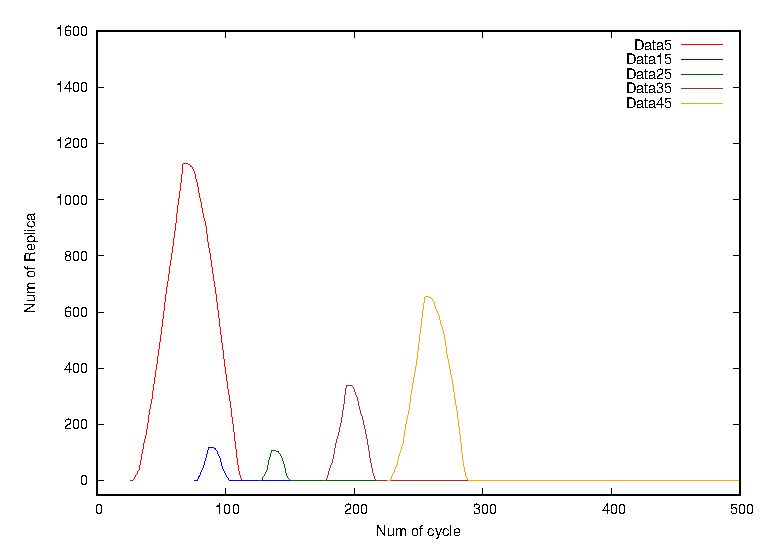
\includegraphics[width=15.0cm]{./figure/owner_counter.eps}
	\end{center}
	\caption{Owner Replicationの,サイクル毎のデータ生存数}
	\label{fig:owner_c}
\end{figure}

\begin{figure}[H]
	\begin{center}
		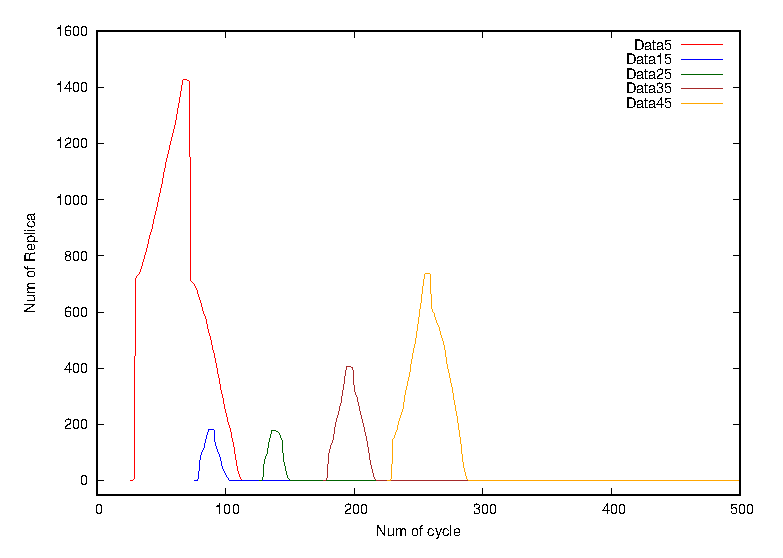
\includegraphics[width=15.0cm]{./figure/path_counter.eps}
	\end{center}
	\caption{Path Replicationの,サイクル毎のデータ生存数}
	\label{fig:path_c}
\end{figure}

\begin{figure}[H]
	\begin{center}
		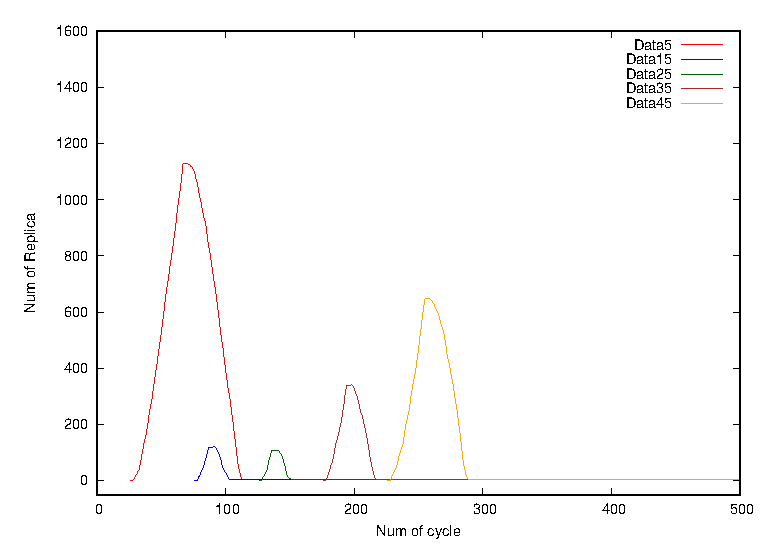
\includegraphics[width=15.0cm]{./figure/relate_counter.eps}
	\end{center}
	\caption{関連研究の提案手法の,サイクル毎のデータ生存数}
	\label{fig:relate_c}
\end{figure}

\begin{figure}[H]
	\begin{center}
		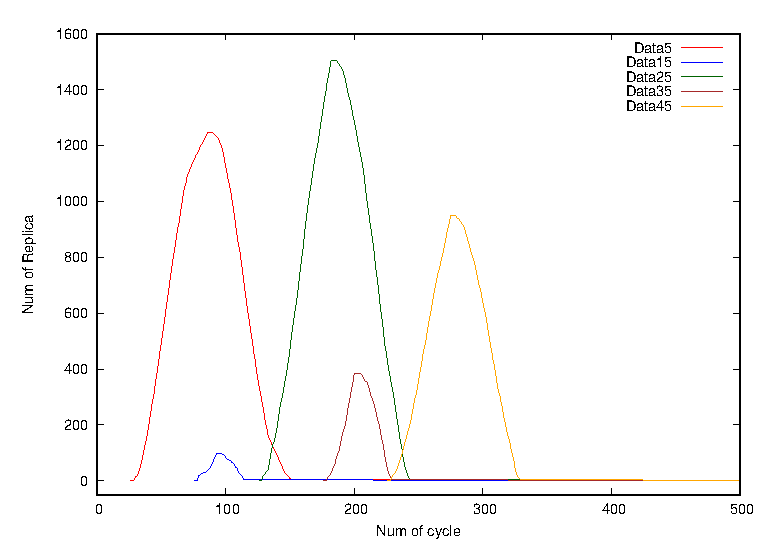
\includegraphics[width=15.0cm]{./figure/cuckoo_counter.eps}
	\end{center}
	\caption{本提案手法の,サイクル毎のデータ生存数}
	\label{fig:cuckoo_c}
\end{figure}

\begin{figure}[H]
	\begin{center}
		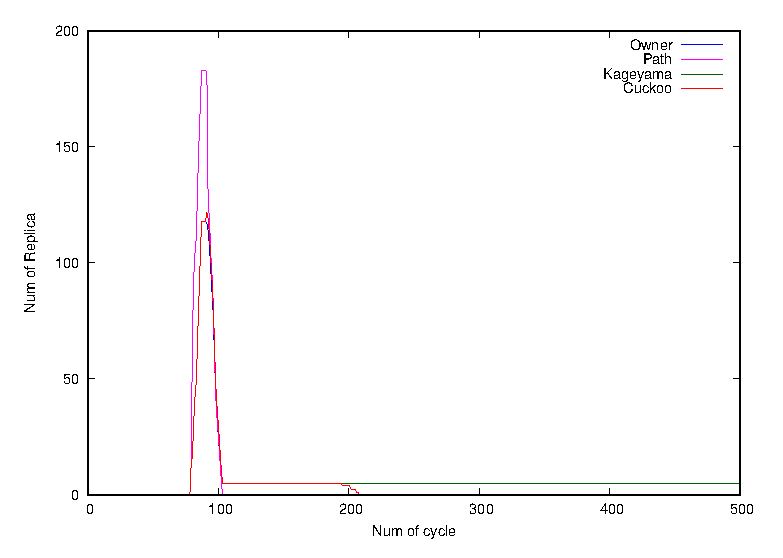
\includegraphics[width=15.0cm]{./figure/counter_comp.eps}
	\end{center}
	\caption{データ35の,複製配置手法ごとの,生存数の推移}
	\label{fig:counter_comp}
\end{figure}

\begin{table}[H]
	\begin{center}
	\caption{低需要データの複製配置開始サイクル}
	\begin{tabular}{ | c | c | c | } \hline
	データ番号 & 複製配置手法 & 開始サイクル数 \\ \hline \hline
	データ5 & 関連研究 & 129 \\ \cline{2-3}
		     & 本提案手法 & 128 \\ \hline
	データ15 & 関連研究 & 97 \\ \cline{2-3}
		     & 本提案手法 & 97 \\ \hline
	データ25 & 関連研究 & 230 \\ \cline{2-3}
		     & 本提案手法 & 229 \\ \hline
	データ35 & 関連研究 & 209 \\ \cline{2-3}
		     & 本提案手法 & 209 \\ \hline
	データ45 & 関連研究 & 314 \\ \cline{2-3}
		     & 本提案手法 & 313 \\ \hline
	\end{tabular}
	\label{tab:counter}
	\end{center}
\end{table}

\newpage
\par 全ての複製配置手法で複製数が上昇し,その後,サイクルが経過するとともに減少していく.これは,それぞれのノードがデータ要求確率に従い,データ要求を行った結果,検索が成功し,それぞれの複製配置手法により,複製が配置されたためである.また,複製数の減少は,ユーザによる削除や,ユーザの離脱による削除が発生したためである.
\par 関連研究の提案手法と本提案手法では,データ要求のあったデータに関しては,Owner Replicationを用いて複製配置を行うため,複製数の増加量は,Owner Replicationに似たものとなっていることが確認できる.減少量に関しては,関連研究の提案手法と,本提案手法では,低需要データの複製配置を別途行っているため,異なることが確認できる.
\par 全ての複製配置手法で,データ15とデータ25の複製数が大きく異なることが確認できる.これは,各ノードのデータ15のデータ要求確率が低く,実際にデータ要求を行うノード数が少ない場合や,データ要求確率に従い,実際にデータ15のデータ要求は発生しているものの,Floodingによる検索で目的のデータが発見できなかった場合や,複製配置されるノードのストレージ残量が,複製配置を行うデータの容量より少ない場合,また,複製配置されるノードが既に,複製配置を行うデータを所持している場合などが考えられる.
\par 図\ref{fig:owner_c},図\ref{fig:path_c},図\ref{fig:counter_comp}より,既存の主な複製配置手法のOwner ReplicationとPath Replicationでは,全てのデータの複製数が0になり,ネットワークから消滅していることが確認できる.これは,既存の主な複製配置手法は,低需要となったデータの生存を考慮していないためである.
\\Owner Replicationに比べ,Path Replicationの複製数が多くなっていくことが確認できる.これは,Owner Replicationは,データ要求を行ったノードにのみ複製配置を行うのに対し,Path Replicationは要求対象のデータを保持するノードから,データ要求を行ったノードに至る経路上のノード全てに複製配置を行うためである.
\par 一方,図\ref{fig:relate_c},図\ref{fig:counter_comp}より,関連研究の提案手法では,全てのデータの複製がネットワークに生存し続けていることが確認できる.これは,関連研究の提案手法が,低需要となったデータの生存を考慮した複製配置が行なっているためである.表\ref{tab:counter}に記したサイクルから,各データの複製配置が開始され,500サイクル経過後も複製数が0になっていないことが確認できる.
\par 図\ref{fig:cuckoo_c},図\ref{fig:counter_comp}より,本提案手法では,全てのデータの複製がネットワークに一定期間生存し続けていることが確認できる.これは,本提案手法が,低需要となったデータの生存を考慮した複製配置を行なっているためである.また,関連研究とは違い,複製配置を開始してから,100サイクル経過する間に,データ要求がなければ複製配置を取りやめるという手法である,そのため,表\ref{tab:counter}に記したサイクルから,各データの複製配置が開始され,100サイクルを過ぎた後減少し,複製数が0になったことが確認できる.

\subsection{サイクル毎の全ノードのストレージ占有率の平均}
図\ref{fig:owner_o}にOwner Replication,図\ref{fig:path_o}にPath Replication,図\ref{fig:relate_o}に関連研究の提案手法,図\ref{fig:cuckoo_o}に本提案手法の,サイクル毎の全ノードのストレージ占有率の平均の結果をそれぞれ記す.また,図\ref{fig:occupancy_comp}に複製配置手法ごとの,全ノードのストレージ占有率の平均の推移を記す.また,表\ref{tab:occupancy}に占有率が増加・減少し,再び1.0になったサイクルを,複製配置手法ごとに記す.

\begin{figure}[H]
	\begin{center}
		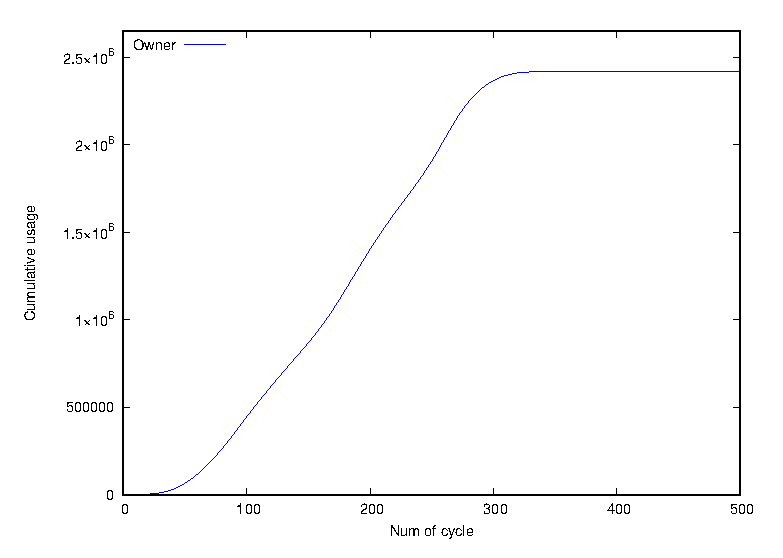
\includegraphics[width=15.0cm]{./figure/owner_occupancy.eps}
	\end{center}
	\caption{Owner Replicationの,サイクル毎の全ノードのストレージ占有率の平均}
	\label{fig:owner_o}
\end{figure}

\begin{figure}[H]
	\begin{center}
		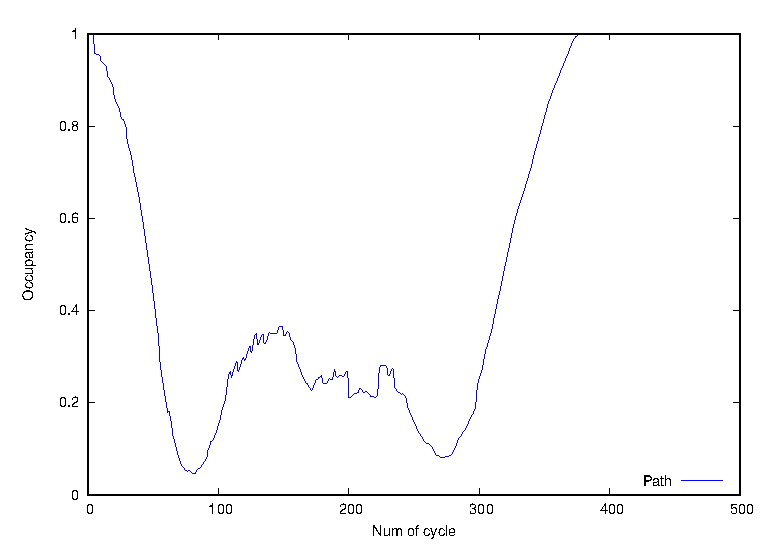
\includegraphics[width=15.0cm]{./figure/path_occupancy.eps}
	\end{center}
	\caption{Path Replicationの,サイクル毎の全ノードのストレージ占有率の平均}
	\label{fig:path_o}
\end{figure}

\begin{figure}[H]
	\begin{center}
		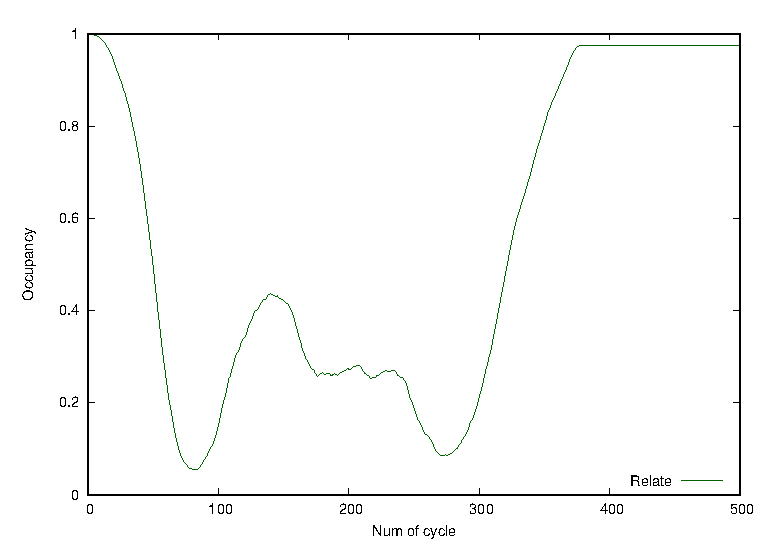
\includegraphics[width=15.0cm]{./figure/relate_occupancy.eps}
	\end{center}
	\caption{関連研究の提案手法の,サイクル毎の全ノードのストレージ占有率の平均}
	\label{fig:relate_o}
\end{figure}

\begin{figure}[H]
	\begin{center}
		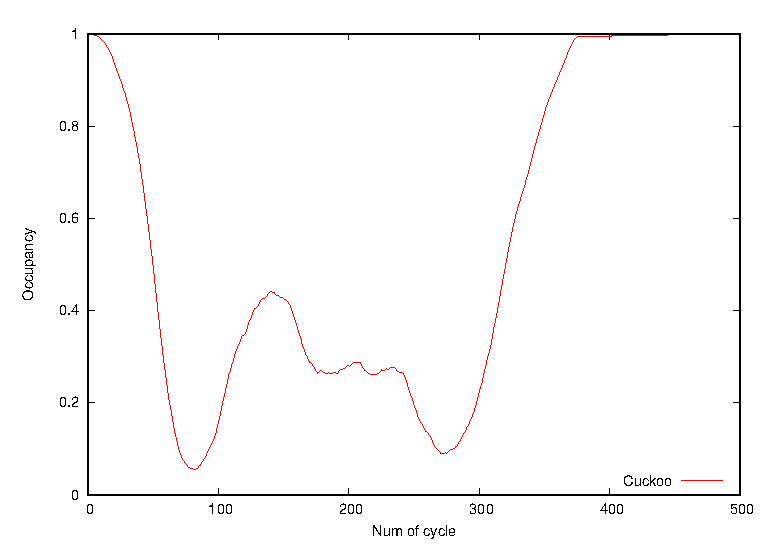
\includegraphics[width=15.0cm]{./figure/cuckoo_occupancy.eps}
	\end{center}
	\caption{本提案手法の,サイクル毎の全ノードのストレージ占有率の平均}
	\label{fig:cuckoo_o}
\end{figure}

\begin{figure}[H]
	\begin{center}
		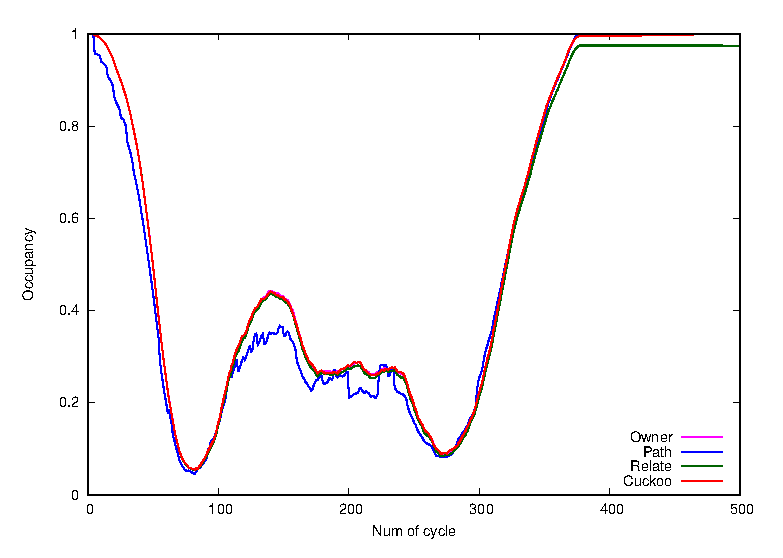
\includegraphics[width=15.0cm]{./figure/occupancy_comp.eps}
	\end{center}
	\caption{複製配置手法ごとの,全ノードのストレージ占有率の平均の推移}
	\label{fig:occupancy_comp}
\end{figure}

\begin{table}[H]
	\begin{center}
	\caption{占有率が再び1.0になるサイクル}
	\begin{tabular}{ | c | c | } \hline
	複製配置手法 & サイクル \\ \hline \hline
	Owner Replication &  379 \\ \hline
    Path Replication & 378  \\ \hline
    関連研究の提案手法 & N/A  \\ \hline
    本提案手法 & 494  \\ \hline
	\end{tabular}
	\label{tab:occupancy}
	\end{center}
\end{table}


\newpage
\par 全ての複製配置手法で,占有率が増減を繰り返し,200サイクル後半を過ぎると一方的に減っていく.これは,データ50個が全てアップロードされ,全種類のデータのデータ要求が無くなり,複製が一方的に減っていくためである.
\par 関連研究の提案手法と本提案手法では,データ要求のあったデータに関しては,Owner Replicationを用いて複製配置を行うため,占有率の増加量は,Owner Replicationに似たものとなっていることが確認できる.減少量に関しては,関連研究の提案手法と,本提案手法では,低需要データの複製配置を別途行っているため異なることが確認できる.
\par 図\ref{fig:owner_o},図\ref{fig:path_o},図\ref{fig:occupancy_comp},表\ref{tab:occupancy}より,Path Replicationは,Owner Replicationに比べ,多くの複製が作成されるため,占有率の増加量が多い.2つの複製配置手法とも,低需要データの生存を考慮していないため,表\ref{tab:occupancy}のサイクルで,全データとその複製がネットワークから消滅し,占有率が再び1.0となっている.
\par 一方,図\ref{fig:relate_o},図\ref{fig:occupancy_comp},表\ref{tab:occupancy}より,関連研究の提案手法では,300サイクル後半から占有率が一定値を保っていることが確認できる.これは,関連研究の提案手法が,低需要となったデータの生存を考慮した複製配置が行なっているため,アップロードされたデータがネットワークに生存し続けており,ノードのストレージを消費しているためである.
\par 図\ref{fig:cuckoo_o},図\ref{fig:occupancy_comp},表\ref{tab:occupancy}より,本提案手法では,Owner Replicationに比べ占有率が高くなっていることが確認できる.これは,本提案手法が,低需要となったデータの生存を考慮した複製配置を行なっているため,一定期間,データがネットワークに生存し,ノードのストレージを消費しているためである.また,関連研究とは違い,複製配置を開始してから,100サイクル経過する間に,データ要求がなければ複製配置を取りやめるという手法であるため,表\ref{tab:occupancy}のサイクルでデータはネットワークから消滅し,占有率は再び1.0になる.

\newpage
\newpage
\subsection{カッコウ探索とFloodingの比較}
表\ref{tab:node}に,複製配置先の選出に,カッコウ探索を用いた本提案手法と,Floodingを行うよう変更した関連研究の提案手法が,実際に選出したノードのバッテリー残量,ストレージ残量の統計の平均を記す.

\begin{table}[H]
	\begin{center}
	\caption{複製配置先に選んだノードの各パラメータの平均値}
	\begin{tabular}{ | c | c | c | } \hline
	選出手法 & パラメータ名 & 平均値 \\ \hline \hline
	カッコウ探索 & バッテリー残量 & 74.43 \\ \cline{2-3}
		     & ストレージ残量 & 7.75 \\ \hline
	Flooding & バッテリー残量 & 68.67 \\ \cline{2-3}
		     & ストレージ残量 & 3.11 \\ \hline
	\end{tabular}
	\label{tab:node}
	\end{center}
\end{table}

\par 表\ref{tab:node}より,両パラメータ共,カッコウ探索を用いた本提案手法が,Floodingを用いるよう変更した関連研究の提案手法より高い値を示していることが確認できる.これは,局所探索を行うFloodingに対し,カッコウ探索は,Levy walkとカッコウ探索のアルゴリズムを用いて広域を探索することができるためであると考えられる.離散値最適化である今回の環境では,良い解を持つノードの,近隣ノードも良い解を持つわけではないため,広域を探索する方が,優れたパラメータを持つノードを発見できると考えれられる.この結果から,カッコウ探索は離散値最適化においても有効であると考えられる.
\par データ要求時の複製配置とは別に,低需要データの複製配置を行うと,ストレージを追加で消費することになる.そのため,データ要求時の複製配置が失敗する回数が増える.表\ref{tab:num}に関連研究の提案手法,本提案手法の,データ要求時に発生する複製配置の,複製配置成功回数と,ストレージ容量不足による複製配置失敗回数を記す.

\begin{table}[H]
	\begin{center}
	\caption{複製配置手法ごとの,複製配置成功・失敗回数}
	\begin{tabular}{ | c | c | c | } \hline
	複製配置手法 & 状態 & 数 \\ \hline \hline
	関連研究の提案手法 & 失敗 & 21693 \\ \cline{2-3}
		     & 成功 & 40769 \\ \hline
    本提案手法 & 失敗 & 20960 \\ \cline{2-3}
		     & 成功 & 41279 \\ \hline
	\end{tabular}
	\label{tab:num}
	\end{center}
\end{table}

\par 表\ref{tab:num}より,本提案手法の方が,成功回数が多く,失敗回数が少ないことが確認できる.これは,表\ref{tab:node}の結果からわかるように,本提案手法の方がストレージ残量の大きいノードに,低需要データの複製を配置してるからであると考えられる.ストレージ残量の大きいノードに,低需要データの複製を配置することにより,そのノードはデータ要求をした際に,ストレージ容量不足による複製配置の失敗が発生しづらくなると考えられる.

\chapter{まとめと今後の課題}
本論文では,データ要求数の少ないデータのネットワークへの生存を考慮した複製配置手法の提案を行い,関連研究の提案手法と,既存複製配置手法との比較を行った.
\par サイクル毎のデータ生存数の比較では,本提案手法は,一定期間,データをネットワークに生存させていることが確認できた.
\par サイクル毎の全ノードのストレージ占有率の平均の比較では,本提案手法は,低需要データの複製配置を行った影響で,Owner Replicationよりも占有率がわずかに高くなり,関連研究の提案手法とは異なり,抵需要データの複製配置を開始したサイクルから,100サイクル経過してもデータ要求がないデータの複製配置を取りやめるという手法により,やがては占有率が1.0になり,ストレージを節約できている事を確認できた.
\par 離散空間のRandom Geometric Graph上で,連続値最適化を対象とするカッコウ探索を用いて離散値最適化を行ったが,カッコウ探索は広域を探索することができるため,局所探索するよりも,良い結果を得ることができた.この結果より,カッコウ探索は離散値最適化においても有効であると考えられる.また,局所探索とのデータ要求時の複製配置の成功数,失敗数の比較において,共に良い結果となった.
\par 今後の課題として,複製配置の際の評価式の改良.バッテリー減少量の改良,また,充電されたケースの追加.ノードの参加・離脱の,仮定・モデルの改良.ネットワークに生存させる,データ要求数の少ないデータの複製数を定める手法の改良が挙げられる.



%%%%%%%%%%%%%%%%%%%%%%%%%%%%%%%%%%%%%%%%%%%%%%%%%%%%%%%%%%%%%%%%%%%%%%%%

%%
%% 謝辞
%%
 \begin{acknowledgements}
 本研究を進めるにあたり,ご指導を頂いた指導教員の林原教授に感謝致します.また日常の議 論を通じて多くの知識や示唆を頂いた同研究室の皆様に感謝します.
 \end{acknowledgements}

%%%%%%%%%%%%%%%%%%%%%%%%%%%%%%%%%%%%%%%%%%%%%%%%%%%%%%%%%%%%%%%%%%%%%%%%

%%
%% 参考文献
%%
\begin{thebibliography}{99}

\bibitem{maruta}
丸田大輔, 山本寛, 尾家祐二."P2Pネットワークにおけるストレージ負荷分散実現のための複製配置手法".電気情報通信学会 信学技報.2004

\bibitem{kageyama}
影山潤, 渋沢進."P2Pネットワークにおけるファイルの消失を防ぐ複製配置手法".DEIM Forum.2009

\bibitem{nomura}
野村浩司, 岩尾忠重, 細川武司, 山田健二."アドホックネットワーク技術への取り組み".FUJITSU.57, 3.2006

\bibitem{jesper}
Jesper Dall, Michael Cristensen."Random Geometric Graphs".Phys. Rev. E 66, 016121.2002

\bibitem{thomas}
Thomas K. Philips, Shivendra S. Panwar, Asser N. Tantawi."Connectivity Properties of a Packet Radio Network Model".IEEE Transactions on Information Theory, vol.35, No.5.1989

\bibitem{yang1}
Xin-She Yang, Suash Deb."Cuckoo Search via Levy flights".Proceeings of World Congress on Nature \& Biologically Inspired Computing (NaBIC 2009, India), IEEE Publications, USA, pp. 210-214

\bibitem{yang2}
Xin-She Yang, Suash Deb."Engineering Optimisation by Cuckoo Search".Int. J. Mathematical Modelling and Numerical Optimisation, vol.1,  No.4, 330-343.2010

\bibitem{ohtani}
大谷紀子 著."進化計算アルゴリズム入門 -生物の行動科学から導く最適解-".オーム社.2018

\bibitem{paul}
Paul Levy."Theorie de L’addition des Variables Aleatoires".Gauthier-Villars.1937

\bibitem{sergey}
Sergey V. Buldyrev, Ary L. Goldberger, Shlomo Havlin, Chung-Kang Peng, Michael Simons, H. Eugene Stanley."Generalized levy-walk model for dna nucleotide sequences".Physical Review E, Vol. 47, No. 6, pp. 4514~4523.1993

\bibitem{andrew}
Andrew M. Edwards, Richard A. Phillips, Nicholas W. Watkins, Mervyn P. Freeman,Eugene J. Murphy, Vsevolod Afanasyev, Sergey V. Buldyrev,M. G. E. da Luz, E. P. Raposo,H. Eugene Stanley, Gandhimohan M. Viswanathan."Revisiting Levy flight search patterns of wandering albatrosses, bumblebees and deer".Nature, Vol. 449, pp. 1044~1048.2007

\bibitem{viswanathan}
G. M. Viswanathan, V. Afanasyev, S. V. Buldyrev, E. J. Murphy, P. A. Prince, H. E. Stanley."Levy flight search patterns of wandering albatrosses".Nature, Vol. 381, pp. 413~415.1996

\bibitem{koyama}
小山英朗, 生天目章."Random Walk と Levy Flight に基づく探索方法の比較". Technical Report 20, 社団法人情報処理学会.2008

\bibitem{nishida}
西田昌彦.グラフ上の "Levy Flight に関する研究".Master’s thesis, 京都産業大学大学院.2016

\bibitem{peersim}
PeerSim: A Peer-to-Peer Simulator."http://peersim.sourceforge.net"

\end{thebibliography}



\end{document}
